\documentclass[12pt, a4paper, twoside]{article}
\usepackage[utf8]{inputenc}
\usepackage{graphicx}
\usepackage{fancyhdr}

\pagestyle{fancy}
\fancyhf{}
\lhead{Mathematisches Pendel}
\rhead{Physik Bericht}

\begin{document}
    \begin{titlepage}
    \begin{center}
        \vspace*{1cm}
        \Huge
        \textbf{Mathematisches Pendel}
 
        \vspace{0.5cm}
        \LARGE
        Physik Kurzbericht
        \vfill
        \normalsize
        Bericht mit Bezug auf das Physikpraktikum vom 10. März 2022  
        \vspace{0.3cm}
      
        Jean \& Aurèle\\
        MNG Rämibühl\\
        24. März 2022
             
    \end{center}
 \end{titlepage}

    \section{Einleitung}
    Unsere Intuition würde uns sagen, dass je schneller sich ein Objekt bewegt, desto schwerer es ist, aber das ist eben nicht der Fall.
    Die direkteste und offensichtlichste Analogie zum Phänomen des Pendels ist das Fallenlassen von Gewichten mit unterschiedlicher Masse
    aus gleicher Höhe; beide kommen zur gleichen Zeit auf dem Boden an (ohne den Widerstand durch die Luftreibung zu berücksichtigen). Nehmen
    wir das Beispiel des Pendels. Nehmen wir an, wir halten das Seil, das die Masse hält, auf Armeslänge. Da sich kein Parameter außer einer
    allmählichen Zunahme der Masse ändert, wird die Kraft, die unser Arm ausübt, um das Gewicht zu halten, immer größer.  Was wir intuitiv als
    höhere Geschwindigkeit wahrnehmen, ist in Wirklichkeit eine höhere Kraft, der wir entgegenwirken müssen. Es war Galileo Galilei, der berühmte
    Astronom, der im Jahr 1590 das folgende Gesetz definierte: Die Anziehungskraft, die die Erde auf eine schwere Masse ausübt, ist stärker als die
    auf eine leichte Masse. Um eine schwere Masse in Bewegung zu setzen, ist jedoch mehr Energie erforderlich: Trägheit. Bei einem Fall gleichen
    sich Anziehung und Trägheit jedoch perfekt aus, sodass die Geschwindigkeit immer gleich bleibt. In der klassischen Gleichung für die Periode
    eines Pendels kommt die Masse übrigens nicht vor. Das Prinzip des Pendels hat viele Entdeckungen ermöglicht. So hat Foucault auf diese Weise
    die Drehbewegung der Erde nachgewiesen. Das Pendel wurde auch verwendet, um die Geschwindigkeit von Geschossen in der Ballistik zu berechnen.
    \vfill
    \section{Bestimmung des Fehlers der Zeitmessung}
    Die Zeit für fünf Schwingungen eines Fadenpendels mit einer Amplitude von 10° wurde 20-mal berechnet. Dabei ergaben sich die folgenden Werte:
    \\
    
      \begin{center}
    \begin{tabular}{l|c|r} % <-- Alignments: 1st column left, 2nd middle and 3rd right, with vertical lines in between
      \textbf{Messung Nr.} & \textbf{Gemessene Zeit} & \textbf{Abweichung}\\
    
      \hline 
      1 & 5.86 s & 0.018 s \\
      2 & 5.88 s & 0.038 s \\
      3 & 5.88 s & 0.038 s \\
      4 & 5.81 s & 0.032 s \\
      5 & 5.83 s& 0.012 s \\
      6 & 5.82 s & 0.022 s \\
      7 & 5.83 s & 0.012 s \\
      8 & 5.78 s & 0.062 s \\
      9 & 5.86 s & 0.018 s \\
      10 & 5.78 s & 0.062 s \\
      11 & 5.92 s & 0.078 s \\
      12 & 5.78 s & 0.062 s \\
      13 & 5.81 s & 0.032 s \\
      14 & 5.83 s & 0.012 s \\
      15 & 5.91 s & 0.068 s \\
      16 & 5.81 s & 0.032 s \\
      17 & 5.89 s & 0.048 s \\
      18 & 5.87 s & 0.028 s \\
      19 & 5.84 s & 0.002 s \\
      20 & 5.85 s & 0.008 s \\

    \end{tabular}
  \end{center}
    Die mittlere Zeit für eine Schwingung entspricht also 5,842 Sekunden.
    Das Fehler der Zeitmessung beträgt 0.078 Sekunden. Dies bedeutet, dass jede Messung mindestens 8 Sekunden dauern muss, damit der Fehler 1\% beträgt.
    \section{Messungen}
    \subsection{Messung A}
    Diese Messung besteht darin, die Schwingungsdauer bei einer konstanten \\ Amplitude und einer konstanten Pendelmasse für zehn verschiedenen Pendellängen zu bestimmen. Die Anzahl Schwingungen ist so gewählt, dass der Fehler weniger als 1\% beträgt. \\
    \\
    \begin{center}
        \begin{tabular}{l|l|c|r|r}
            \textbf{Pendellänge} & \textbf{Anzahl Schwingungen} & \textbf{1. Messung} & \textbf{2. Messung} & \textbf{Schwingungsdauer}\\ 

            \hline
            10 \textit{cm} & 13 & 8.35 \textit{s} & 8.22 \textit{s} & 0.6370 \textit{s} \\ 
            20 \textit{cm} & 10 & 9.13 \textit{s} & 8.90 \textit{s} & 0.9015 \textit{s} \\ 
            30 \textit{cm} & 9 & 10.12 \textit{s} & 10.00 \textit{s} & 1.1180 \textit{s} \\ 
            40 \textit{cm} & 8 & 10.32 \textit{s} & 10.21 \textit{s} & 1.2830 \textit{s} \\ 
            50 \textit{cm} & 9 & 12.89 \textit{s} & 12.98 \textit{s} & 1.4338 \textit{s} \\ 
            60 \textit{cm} & 6 & 9.75 \textit{s} & 9.46 \textit{s} & 1.6008 \textit{s} \\ 
            70 \textit{cm} & 6 & 10.31 \textit{s} & 10.31 \textit{s} & 1.7187 \textit{s} \\ 
            80 \textit{cm} & 5 & 9.13 \textit{s} & 9.14 \textit{s} & 1.8270 \textit{s} \\ 
            90 \textit{cm} & 5 & 9.71 \textit{s} & 9.62 \textit{s} & 1.9330 \textit{s} \\ 
            100 \textit{cm} & 5 & 10.11 \textit{s} & 10.03 \textit{s} & 2.0140 \textit{s} \\ 

          \end{tabular}
    \end{center}
    \subsection{Messung B}
    Hier wurde mit gleicher Pendellänge und Amplitude die Schwingungsdauer von Pendeln mit drei unterschiedlichen Massen. Es wird immer noch genug lang gemessen, um ein Fehler von weniger als 1\% zu haben.
    Die Länge des Pendels \textit{l = 50 cm} und die Amplitude \textit{$\alpha$ = 20°} sind fix.
    \begin{center}
        \begin{tabular}{l|l|c|r|r}
            \textbf{Pendelmasse} & \textbf{Anzahl Schwingungen} & \textbf{1. Messung} & \textbf{2. Messung} & \textbf{Schwingungsdauer}\\

            \hline
            101,5 \textit{g} & 9 & 12,85 \textit{s} & 12,98 \textit{s} & 1,435 \textit{s}\\
            358 \textit{g} & 8 & 11,20 \textit{s} & 11,20 \textit{s} & 1,40 \textit{s}\\
            33,5 \textit{g} & 8 & 11,32 \textit{s} & 11,46 \textit{s} & 1,42 \textit{s}\\
        \end{tabular}
    \end{center}
    \subsection{Messung C}
    Das Ziel dieser Messung ist es, ein Beschloss über den Einfluss der Amplitude zu ziehen. Es wurden 2 verschiedene Amplituden gewählt. Für je eine wurden zwei Messungen durchgeführt. Die Länge des Pendels \textit{l = 50 cm} und die Masse \textit{m = 358 g} sind festgelegt.
    \begin{center}
        \begin{tabular}{l|l|c|r|r}
            \textbf{Amplitude} & \textbf{Anzahl Schwingungen} & \textbf{1. Messung} & \textbf{2. Messung} & \textbf{Schwingungsdauer}\\
            \hline
            20 ° & 8 & 11,20 \textit{s} & 11,20 \textit{s} & 1,40 \textit{s}\\
            40 ° & 8 & 11,94 \textit{s} & 11,96 \textit{s} & 1,49375 \textit{s}\\
        \end{tabular}
    \end{center}
    Man stellt fest, dass wenn die Amplitude sich um 20° ändert, es fast $\frac{1}{10}$ Sekunden Unterschied gibt.
    \section{Aufgaben}
    \subsection{Aufgabe 2}
    \begin{figure}[h]
        \begin{center}
            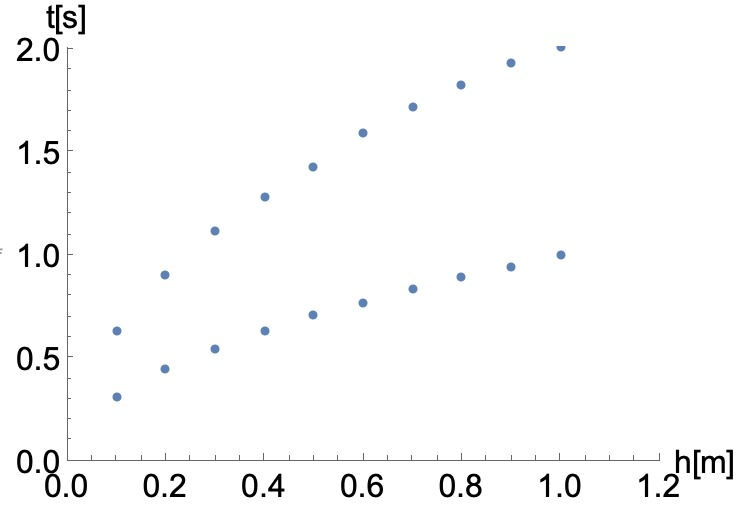
\includegraphics[width=8cm]{aufgabe2.png}
            \caption{Grafik}
            \label{fig:figure1}        
        \end{center}
    \end{figure}
    \subsection{Aufgabe 3}

\end{document}